\documentclass{sig-alternate}

\usepackage{url}
\newtheorem{example}{Example}
\newtheorem{definition}{Definition}
%%%%%% Non recom packages
\usepackage{pst-node}
\usepackage{pst-rel-points}
%%%%%%%%%%%%%%%%%%%%%%%%%%%%%%%%%%%%%%%%
%%%%%%% New Commands %%%%%%%%%%%%%%%%%%
%%%%%%%%%%%%%%%%%%%%%%%%%%%%%%%%%%%%%%%%
\newcommand{\cmt}[1]{} % commented out stuff
\newcommand{\is}{\itemsep -1mm} % reduce space between items
\newcommand{\hide}[1]{} % hidden for double blind review

% Review these names
\newcommand{\p}{\ensuremath{p}}
\newcommand{\q}{\ensuremath{q}}
\newcommand{\s}{\ensuremath{s}}
\newcommand{\myr}{\ensuremath{r}}

\newcommand{\B}{\mbox{\tt B}}
\renewcommand{\a}{\mbox{\tt a}}
\renewcommand{\b}{\mbox{\tt b}}
\renewcommand{\c}{\mbox{\tt c}}
\renewcommand{\d}{\mbox{\tt d}}
\newcommand{\m}{\mbox{\tt m}}

\newcommand{\drct}{\ensuremath{D}}
\newcommand{\indrct}{\ensuremath{I}}
\newcommand{\heap}{\ensuremath{\mathcal{H}}}
\newcommand{\fields}{\ensuremath{\mathcal{F}}}
\newcommand{\upath}{\ensuremath{\mathcal{U}}}
\newcommand{\shape}{\mbox{shape}}
\newcommand{\nat}{\ensuremath{\mathcal{N}}}

\newcommand{\mwedge}{\; \wedge \;}
\newcommand{\mvee}{\; \vee \;}
\newcommand{\mcup}{\; \cup \;}
\newcommand{\mjoin}{\; \Join \;}
\newcommand{\mbackslash}{\; \backslash \;}
\newcommand{\subC}{\mbox{\scalebox{0.6}{\Cycle}}}
\newcommand{\subD}{\mbox{\scalebox{0.6}{\Dag}}}

\newcommand{\epsilonset}{\ensuremath{\{\epsilon\}}}
\newcommand{\epsilonpairset}{\ensuremath{\{\epsilon,\epsilon\}}}

\newcommand{\dout}{\mbox{\footnotesize\em out}}
\newcommand{\din}{\mbox{\footnotesize\em in}}
\newcommand{\dkill}{\mbox{\footnotesize\em kill}}
\newcommand{\dgen}{\mbox{\footnotesize\em gen}}

\newcommand{\GenC}[1]{\ensuremath{{#1}_{\subC}^{\dgen}}}
\newcommand{\GenD}[1]{\ensuremath{{#1}_{\subD}^{\dgen}}}
\newcommand{\KillC}[1]{\ensuremath{{#1}_{\subC}^{\dkill}}}
\newcommand{\KillD}[1]{\ensuremath{{#1}_{\subD}^{\dkill}}}
\newcommand{\InC}[1]{\ensuremath{{#1}_{\subC}^{\din}}}
\newcommand{\InD}[1]{\ensuremath{{#1}_{\subD}^{\din}}}
\newcommand{\OutC}[1]{\ensuremath{{#1}_{\subC}^{\dout}}}
\newcommand{\OutD}[1]{\ensuremath{{#1}_{\subD}^{\dout}}}

\newcommand{\merge}{\ensuremath{\mathrm{merge}}}
\newcommand{\project}[2]{\ensuremath{#1\triangleright\!\!#2}}
\newcommand{\num}[1]{\ensuremath{|#1|}}
\newcommand{\remOne}[2]{\ensuremath{#1 \ominus #2}}
\newcommand{\remAll}[2]{\ensuremath{#1\uminus #2}}

\newcommand{\Gen}[1]{{\mbox{{\tt gen}}_{\mbox{\scalebox{0.6}{{\tt #1}}}}}}
\newcommand{\Kill}[1]{{\mbox{{\tt kill}}_{\mbox{\scalebox{0.6}{{\tt #1}}}}}}
\newcommand{\mb}[1]{\mbox{{\tt #1}}}
%\newcommand{\DFM}[2]{\mb{$D_F$}[\mb{#1},\mb{#2}]}
%\newcommand{\IFM}[2]{\mb{$I_F$}[\mb{#1},\mb{#2}]}
\newcommand{\DFM}[2]{\ensuremath{D_F[#1,#2]}}
\newcommand{\IFM}[2]{\ensuremath{I_F[#1,#2]}}
\newcommand{\Tree}{{\tt Tree}}
\newcommand{\Dag}{{\tt Dag}}
\newcommand{\Cycle}{{\tt Cycle}}
\newcommand{\upstmt}[1]{{\tt p$\rightarrow$f = #1}}
\newcommand{\TV}{{\tt TrueVars}}
\newcommand{\fieldD}[2]{\ensuremath{{#1}_{#2}^\drct}}
\newcommand{\fieldI}[3]{\ensuremath{{#1}_{#2}^{\indrct#3}}}
\newcommand{\range}[3]{\ensuremath{{#1} \leq {#2} \leq {#3}}}
\newcommand{\U}{{\rm Unknown}}
\newcommand{\fig}[1]{\includegraphics[scale=.5]{#1}}
\newcommand{\false}{\textbf{False}}
\newcommand{\true}{\textbf{True}}

\newcommand{\sub}[2]{\ensuremath{{#1}_{#2}}}
%\renewcommand{\green}{\blue}

\begin{document}
%
% --- Author Metadata here ---
\conferenceinfo{SAC'12}{March 25-29, 2012, Riva del Garda, Italy.}
\CopyrightYear{2011} % Allows default copyright year (2002) to be over-ridden - IF NEED BE.
\crdata{978-1-4503-0857-1/12/03}  % Allows default copyright data (X-XXXXX-XX-X/XX/XX) to be over-ridden.
% --- End of Author Metadata ---

\title{Precise Shape Analysis using Field Sensitivity}
\hide{author information}

\maketitle
\begin{abstract}
Programs in high level languages make intensive use of heap
to support dynamic data structures.  Analyzing these programs
requires precise reasoning about the heap structures. Shape
analysis refers to the class of techniques that statically
approximate the run-time structures created on the heap.  In
this paper, we present a novel field sensitive shape analysis
technique to identify the shapes of the heap structures.  The
novelty of our approach lies in the way we use field
information to remember the paths that result in a particular
shape (Tree, DAG, Cycle).  We associate the field information
with a shape in two ways: (a) through boolean functions that
capture the shape transition due to change in a particular
field, and (b) through matrices that store the field
sensitive path information among two pointer variables.  This
allows us to easily identify transitions from Cycle to DAG,
from Cycle to Tree and from DAG to Tree, thus making the
shape more precise.
\end{abstract}

% A category with the (minimum) three required fields
\category{F.2.0}{Analysis of Algorithms and Problem Complexity}{General}
%A category including the fourth, optional field follows...
\category{D.3.4}{Programming Languages}{Processors }[Compilers]
\category{D.2.4}{Software Engineering}{Software/Program Verification}[Formal methods]
\category{E.1}{Data}{Data Structures}[Graphs and networks, trees]
\category{F.3.1}{Logics and Meanings of Programs}{Specifying and Verifying and Reasoning about Programs}[Logics of programs ]
\category{F.3.2}{Logics and Meanings of Programs}{Semantics of Programming Languages}[Program Analysis]
%%
\terms{Algorithms, Languages, Verification, Theory}
%%
\keywords{Shape analysis, dataflow analysis, pointer analysis, static analysis, heap analysis} % NOT required for Proceedings

%%%%%%%%%%%%%%%%%%%%%%%%%%%%%%%%%%%%%%%%%%%%%%%%%%%%%
\section{Introduction}
%%%%%%%%%%%%%%%%%%%%%%%%%%%%%%%%%%%%%%%%%%%%%%%%%%%%%
Shape analysis is the term for the class of static analysis
techniques that are used to infer useful properties about
heap data and the programs manipulating the heap. The shape
information of a data structure accessible from a heap
directed pointer can be used for disambiguating heap accesses
originating from that pointer. This is useful for variety of
applications, for e.g. compile time optimizations,
compile-time garbage collection, debugging, verification,
instruction scheduling and parallelization.

In the last two decades, several shape analysis techniques have
been proposed in literature. However, there is a trade-off
between speed and precision for these techniques. Precise
shape analysis
algorithms~\cite{Sagiv96,shaham03heap,distefano06local,hackett05region} 
are not practical as they do not scale to the size of complex
heap manipulating programs. To achieve scalability,
the practical shape analysis
algorithms~\cite{Chase90,Ghiya96,marron06static} trade
precision for speed.

In this paper, we present a shape analysis technique that
uses limited field sensitivity to infer the shape of the
heap. The novelty of our approach lies in the way we use
field information to remember the paths that result in a
particular shape (Tree, DAG, Cycle).  This allows us to
identify transitions from a conservative shape to a more precise
shape (i.e., from Cycle to DAG, from Cycle to Tree and from
DAG to Tree) due to destructive updates. This in turn enables
us to infer precise shape information.


The field sensitivity information is captured in two ways:
(a) we use field based boolean variables to remember the
direct connections between two pointer variables, and (b) we
compute field sensitive matrices that store the approximate
path information between two pointer variable. We generate
boolean functions at each program point that use the above
field sensitive information to infer the shape of the pointer
variables.

We discuss some of the prior works on shape analysis in
Sect.~\ref{sec:bgrel}. A motivating example is used in
Sect.~\ref{sec:motiv} to explain the intuition behind our
analysis .  The analysis is formalized in
Sect.~\ref{sec:Formal_Definitions} that describes the
notations used and in Sect.~\ref{sec:Analysis_Rules} that
gives the analysis rules. Some properties of our analysis
are described in
Sect.~\ref{sec:props}. Section~\ref{sec:concl} concludes the
presentation and gives directions for future work.

%%%%%%%%%%%%%%%%%%%%%%%%%%%%%%%%%%%%%%%%%%%%%%%%%%%%%
\section{Related Work}\label{sec:bgrel}
%%%%%%%%%%%%%%%%%%%%%%%%%%%%%%%%%%%%%%%%%%%%%%%%%%%%%

The shape-analysis problem was initially studied in the
context of functional languages. Jones and
Muchnick~\cite{Jones79} proposed one of the earliest shape
analysis technique for Lisp-like languages with destructive
updates of structure. They used sets of finite shape graphs
at each program point to describe the heap structure.  To
keep the shape graphs finite, they introduced the concept of
$k$-limited graphs where all nodes beyond $k$ distance from
root of the graph are summarized into a single node. Hence
the analysis resulted in conservative approximations. The
analysis is not practical as it is extremely costly both in
time and space .
%
Chase et.~al.~\cite{Chase90} introduced the concept of limited
reference count to classify heap objects into different
shapes. They also classified the nodes in concrete and
summary nodes, where summary nodes were used to guarantee
termination. Using the reference count and concreteness
information of the node, they were able to kill relations
({\em strong updates}) for assignments of the form $\p\rightarrow f = \q$
in some cases. However, this information is not
insufficient to compute precise shape, and detects false
cycle even in case of simple algorithms like destructive list
reversal.

Sagiv et.~al.~\cite{Sagiv96,Sagiv02toplas} proposed
generic, unbiased shape analysis algorithms based on {\em
  Three-Valued} logic. They introduce the concepts of {\em
  abstraction} and {\em re-materialization}. Abstraction is
the process of summarizing multiple nodes into one and is
used to keep the information bounded.  Re-materialization is
the process of obtaining concrete nodes from summary node and
is required to handle destructive updates. By identifying
suitable predicates to track, the analysis can be made very
precise.  However, the technique has potentially exponential
run-time in the number of predicates, and therefore not
suitable for large programs.
%
Distefano et.~al.~\cite{distefano06local} presented a shape
analysis technique for linear data structures (linked-list
etc.), which works on symbolic execution of the whole program
using separation logic. Their technique works on suitable
abstract domain, and guarantees termination by converting
symbolic heaps to finite canonical forms, resulting in a
fixed-point. By using enhanced abstraction scheme and
predicate logic, Cherini et.~al.~\cite{cherini10shape}
extended this analysis to support nonlinear data structure
(tree, graph etc.).

Berdine et.~al.~\cite{berdine07shape} proposed a method
    for identifying composite data structures using generic
    higher-order inductive predicates and parameterized
    spatial predicates.  However, using of separation logic
    does not perform well in inference of heap properties.
Hackett and Rugina in~\cite{hackett05region} presented a new
approach for shape analysis which reasons about the state of
a single heap location independently. This results in precise
abstractions of localized portions of heap. This local
reasoning is then used to reason about global heap using
context-sensitive interprocedural analysis.  Cherem
et.~al.~\cite{cherem07doubly} use the local abstraction
scheme of~\cite{hackett05region} to generate local invariants
to accurately compute shape information for complex data
structures.
%
Jump and McKinley~\cite{maria09dynamic} give a technique for
dynamic shape analysis that characterizes the shape of
recursive data structure in terms of dynamic degree metrics
which uses in-degrees and out-degrees of heap nodes to
categorize them into classes. While this technique is useful
for detecting certain types of errors; it fails to visualize
and understand the shape of heap structure and cannot express
the sharing information in general.

Our work is closest to the work proposed by Ghiya
et.~al.~\cite{Ghiya96} and by Marron
et.~al.~\cite{marron06static}.  Ghiya et.~al.~\cite{Ghiya96}
keeps interference and direction matrices between any two
pointer variables pointing to heap object and infer the shape
of the structure as Tree, DAG or Cycle. They have
demonstrated the practical applications of their
analysis~\cite{Ghiya98a,Ghiya98b}
and shown that it works well on practical programs.  The main
shortcoming of this approach is that it cannot handle kill
information. In particular, the approach is unable to
identify transitions from Cycle to DAG, from Cycle to Tree
and from DAG to Tree, and hence conservatively identify the
shapes.
%
Marron et.~al.~\cite{marron06static} presents a data flow
framework that uses heap graphs to model data flow
values. The analysis uses technique similar to
re-materialization, but unlike parametric shape analysis
techniques~\cite{Sagiv02toplas}, the
re-materialization is approximate and may result in loss of
precision. 

Our method is based on data flow analysis that uses matrices
and boolean functions as data flow values. We use field
sensitive matrices to store path information, and boolean
variables to record field updates. By incorporating field
sensitivity information, we are able to improve the precision
without much impact on efficiency. The next section presents
a simplified view of our approach before we explain it in
full details.

%%%%%%%%%%%%%%%%%%%%%%%%%%%%%%%%%%%%%%%%%%%%%%%%%%%%%
\section{A Motivating Example}\label{sec:motiv}
%%%%%%%%%%%%%%%%%%%%%%%%%%%%%%%%%%%%%%%%%%%%%%%%%%%%%

Following the
literature~\cite{Ghiya96,Sagiv96,marron06static},
we define the shape attribute for a pointer $\p$
as:
\begin{eqnarray*}
  \p.\shape = \left\{ \begin{array}{@{}rl@{}}
    \Cycle & \mbox{If a cycle can be reached from $\p$} \\ 
    \Dag & \mbox{Else if a DAG can be reached from $\p$} \\
    \Tree & \mbox{Otherwise} \\
  \end{array} \right.
\end{eqnarray*}
where the heap is visualized as a directed graph, and cycle
and DAG have there natural graph-theoretic meanings. For each
pointer variable, our analysis computes the shape attribute
of the data structure pointed to by the variable.  We use the
code fragment in Fig.~\ref{fig:motiv}(a) to motivate the need
for a field sensitive shape analysis.
\begin{example}{\rm
\begin{figure*}[t]
\centering
  \begin{tabular}{@{}lcc@{}}
\begin{tabular}[b]{l}
\scalebox{0.80}{\small\tt
      \begin{tabular}[b]{l}
        S1. p = malloc(); \\
        S2. q = malloc(); \\
        S3. p$\rightarrow$f = q; \\
        S4. p$\rightarrow$h = q; \\
        S5. q$\rightarrow$g = p; \\
        S6. q$\rightarrow$g = NULL;   \\
        S7. p$\rightarrow$h = NULL; 
      \end{tabular}
    } \\ 
\scalebox{0.80}{(a) A code fragment} \\ \\
\scalebox{0.76}{  \begin{tabular}[b]{|cc|l|l|l|} \hline
    {\bf After} && $f_{pq}$ & $h_{pq}$ & $g_{qp}$ \\
    {\bf Stmt} && & &     \\ \hline
    {\tt S1 } && false & false & false \\
    {\tt S2 } && false & false & false \\
    {\tt S3 } && true  & false & false \\
    {\tt S4 } && true  & true  & false \\
    {\tt S5 } && true  & true  & true  \\
    {\tt S6 } && true  & true  & false \\
    {\tt S7 } && true  & false & false \\ \hline
  \end{tabular}}
\end{tabular}
&
\hspace{-1mm}\scalebox{0.69}{\begin{tabular}[b]{|l|@{}c@{}|@{}c@{}|}
    \hline
{\bf After} & $D$ & $I$ \\
 {\bf Stmt} & & \\ \hline
{\tt S1}
& \begin{tabular}{|c|cc|}
{\tt } & $\p$  &  $\q$ \\ \hline
$\p$ & 1  & 0 \\
$\q$ & 0  & 0\\
\hline
\end{tabular} &
\begin{tabular}{|c|cc|}
{\tt } & $\p$  &  $\q$ \\ \hline
$\p$ & 1  & 0 \\
$\q$ & 0  & 0\\
\hline
\end{tabular}\\ \hline
{\tt S2}
& \begin{tabular}{|c|cc|}
{\tt } & $\p$  &  $\q$ \\ \hline
$\p$ & 1  & 0 \\
$\q$ & 0  & 1\\
\hline
\end{tabular}&
\begin{tabular}{|c|cc|}
{\tt } & $\p$  &  $\q$ \\ \hline
$\p$ & 1  & 0 \\
$\q$ & 0  & 1\\
\hline
\end{tabular} \\ \hline
{\tt S3}
 & \begin{tabular}{|c|cc|} \hline 
{\tt } & $\p$  &  $\q$ \\ \hline
$\p$ & 1  & 1 \\
$\q$ & 0  & 1\\
\hline
\end{tabular}&
\begin{tabular}{|c|cc|} \hline 
{\tt } & $\p$  &  $\q$ \\ \hline
$\p$ & 1  & 1 \\
$\q$ & 1  & 1\\
\hline
\end{tabular}\\ \hline
{\tt S4}
 & \begin{tabular}{|c|cc|} \hline 
{\tt } & $\p$  &  $\q$ \\ \hline
$\p$ & 1  & 1 \\
$\q$ & 0  & 1\\
\hline
\end{tabular} &
\begin{tabular}{|c|cc|} \hline 
{\tt } & $\p$  &  $\q$ \\ \hline
$\p$ & 1  & 1 \\
$\q$ & 1  & 1\\
\hline
\end{tabular}\\ \hline
{\tt S5}
 & \begin{tabular}{|c|cc|} \hline 
{\tt } & $\p$  &  $\q$ \\ \hline
$\p$ & 1  & 1 \\
$\q$ & 1  & 1\\
\hline
\end{tabular} &
\begin{tabular}{|c|cc|} \hline 
{\tt } & $\p$  &  $\q$ \\ \hline
$\p$ & 1  & 1 \\
$\q$ & 1  & 1\\
\hline
\end{tabular} 
\\ \hline
{\tt S6}
 & \begin{tabular}{|c|cc|} \hline 
{\tt } & $\p$  &  $\q$ \\ \hline
$\p$ & 1  & 1 \\
$\q$ & 1  & 1\\
\hline
\end{tabular} &
\begin{tabular}{|c|cc|} \hline 
{\tt } & $\p$  &  $\q$ \\ \hline
$\p$ & 1  & 1 \\
$\q$ & 1  & 1\\
\hline
\end{tabular} 
\\ \hline
{\tt S7}
 & \begin{tabular}{|c|cc|} \hline 
{\tt } & $\p$  &  $\q$ \\ \hline
$\p$ & 1  & 1 \\
$\q$ & 1  & 1\\
\hline
\end{tabular} &
\begin{tabular}{|c|cc|} \hline 
{\tt } & $\p$  &  $\q$ \\ \hline
$\p$ & 1  & 1 \\
$\q$ & 1  & 1\\
\hline
\end{tabular} 
\\ \hline
\end{tabular}} &
\hspace{-1mm}\scalebox{0.69}{
\begin{tabular}[b]{|l@{}|@{}c@{}|@{}c@{}|} \hline
 {\bf After} & $D_F$ & $I_F$ \\ 
 {\bf Stmt} & & \\ \hline

{\tt S1} & 
\begin{tabular}{|p{3mm}|p{12mm}p{12mm}|} \hline 
  & $\p$  &  $\q$ \\ \hline
  $\p$ & $\left\{\epsilon\right\}$  & $\emptyset$ \\
  $\q$ & $\emptyset$  & $\emptyset$\\
  \hline
\end{tabular} &
\begin{tabular}{|p{3mm}|p{28mm}p{28mm}|} \hline 
  & $\p$  &  $\q$ \\ \hline
  $\p$ & $\left\{(\epsilon, \epsilon)\right\}$  & $\emptyset$ \\
  $\q$ & $\emptyset$  & $\emptyset$\\
  \hline
\end{tabular} \\ \hline

{\tt S2} & 
\begin{tabular}{|p{3mm}|p{12mm}p{12mm}|} \hline 
  & $\p$  &  $\q$ \\ \hline
  $\p$ & $\left\{\epsilon\right\}$  &    $\emptyset$ \\
  $\q$ &    $\emptyset$       & $\left\{\epsilon\right\}$\\
  \hline
\end{tabular} &
\begin{tabular}{|p{3mm}|p{28mm}p{28mm}|} \hline 
  & $\p$  &  $\q$ \\ \hline
  $\p$ & $\left\{(\epsilon, \epsilon)\right\}$  & $\emptyset$ \\
  $\q$ &        $\emptyset$  & $\left\{(\epsilon, \epsilon)\right\}$\\
  \hline
\end{tabular} \\ \hline

{\tt S3} &
\begin{tabular}{|p{3mm}|p{12mm}p{12mm}|} \hline 
  & $\p$  &  $\q$ \\ \hline
  $\p$ & $\left\{\epsilon\right\}$  &    $\left\{f\right\}$ \\
  $\q$ &    $\emptyset$       & $\left\{\epsilon\right\}$\\
  \hline
\end{tabular} &
\begin{tabular}{|p{3mm}|p{28mm}p{28mm}|} \hline 
  & $\p$  &  $\q$ \\ \hline
  $\p$ & $\left\{(\epsilon, \epsilon)\right\}$  & $\left\{(f, \epsilon)\right\}$ \\
  $\q$ &        $\left\{(\epsilon, f)\right\}$  & $\left\{(\epsilon, \epsilon)\right\}$\\
  \hline
\end{tabular} \\ \hline

{\tt S4} &
\begin{tabular}{|p{3mm}|p{12mm}p{12mm}|} \hline 
  & $\p$  &  $\q$ \\ \hline
  $\p$ & $\left\{\epsilon\right\}$  &    $\left\{f, h\right\}$ \\
  $\q$ &    $\emptyset$       & $\left\{\epsilon\right\}$\\
  \hline
\end{tabular} &
\begin{tabular}{|p{3mm}|p{28mm}p{28mm}|} \hline 
  & $\p$  &  $\q$ \\ \hline
  $\p$ & $\left\{(\epsilon, \epsilon)\right\}$  & $\left\{(f, \epsilon), (h, \epsilon)\right\}$ \\
  $\q$ &        $\left\{(\epsilon, f), (\epsilon, h)\right\}$  & $\left\{(\epsilon, \epsilon)\right\}$\\
  \hline 
\end{tabular} \\ \hline

{\tt S5} &
\begin{tabular}{|p{3mm}|p{12mm}p{12mm}|} \hline 
  & $\p$  &  $\q$ \\ \hline
  $\p$ & $\left\{\epsilon, f, h\right\}$ &    $\left\{f, h\right\}$ \\ 
  $\q$ &    $\left\{g\right\}$       & $\left\{\epsilon, g\right\}$\\ 
  \hline
\end{tabular} &
\begin{tabular}{|p{3mm}|p{28mm}p{28mm}|} \hline 
  & $\p$  &  $\q$ \\ \hline
  $\p$ & $\left\{(\epsilon, \epsilon)\right\}$  & 
  $\left\{(f, \epsilon), (h, \epsilon),  (\epsilon, g)\right\}$ \\ 
  $\q$ &        $\left\{(\epsilon, f), (\epsilon, h), (g, \epsilon)\right\}$
  & $\left\{(\epsilon, \epsilon)\right\}$ \\ 
  \hline
\end{tabular} \\ \hline

{\tt S6}&
\begin{tabular}{|p{3mm}|p{12mm}p{12mm}|} \hline 
  & $\p$  &  $\q$ \\ \hline
  $\p$ & $\left\{\epsilon\right\}$  &    $\left\{f, h\right\}$ \\
  $\q$ &   $\emptyset$       & $\left\{\epsilon\right\}$\\
  \hline
\end{tabular} &
\begin{tabular}{|p{3mm}|p{28mm}p{28mm}|} \hline 
  & $\p$  &  $\q$ \\ \hline
  $\p$ & $\left\{(\epsilon, \epsilon)\right\}$  & $\left\{(f, \epsilon), (h, \epsilon)\right\}$ \\
  $\q$ &        $\left\{(\epsilon, f), (\epsilon, h)\right\}$  & $\left\{(\epsilon, \epsilon)\right\}$\\
  \hline
\end{tabular} \\ \hline

{\tt S7} &
\begin{tabular}{|p{3mm}|p{12mm}p{12mm}|} \hline 
  & $\p$  &  $\q$ \\ \hline
  $\p$ & $\left\{\epsilon\right\}$  &    $\left\{f\right\}$ \\
  $\q$ &    $\emptyset$       & $\left\{\epsilon\right\}$\\
  \hline
\end{tabular} &
\begin{tabular}{|p{3mm}|p{28mm}p{28mm}|} \hline 
  & $\p$  &  $\q$ \\ \hline
  $\p$ & $\left\{(\epsilon, \epsilon)\right\}$  & $\left\{(f, \epsilon)\right\}$ \\
  $\q$ &        $\left\{(\epsilon, f)\right\}$  & $\left\{(\epsilon, \epsilon)\right\}$\\
  \hline
\end{tabular} \\ \hline 
\end{tabular}}
\\ 
\scalebox{0.80}{(d) \begin{tabular}[t]{@{}p{23mm}}
    Boolean Variables and their values
  \end{tabular}} & 
\scalebox{0.80}{(b) \begin{tabular}[t]{@{}p{23mm}}
             Direction ($D$) and Interference ($I$) matrices~\cite{Ghiya96}
         \end{tabular}} &
\scalebox{0.80}{(c) \begin{tabular}[t]{@{}p{43mm}} Field Sensitive Direction ($D_F$) and
  Interference ($I_F$) matrices.
  \end{tabular}
} 
  \end{tabular}
\caption{A motivating example\label{fig:motiv}}
\end{figure*}

Consider the code segment in the Fig.~\ref{fig:motiv}(a),
At {\tt S4}, a DAG is created that is reachable from $\p$. 
At {\tt S5}, a cycle is created that is reachable from
both $\p$ and $\q$. This cycle is destroyed at line
{\tt S6} and the DAG is destroyed at {\tt S7}.

Field insensitive shape analysis algorithms use conservative
kill information and hence they are, in general, unable to
infer the shape transition from cycle to DAG or from DAG to
Tree.  For example, the algorithm by Ghiya
et.~al.~\cite{Ghiya96} can correctly report the shape
transition from DAG to cycle\ (at {\tt S5}), but fails to
infer the shape transition from cycle to DAG (at {\tt S6})
and from DAG\ to \Tree\ (at {\tt S7}). This is evident from
Fig.~\ref{fig:motiv}(b) that shows the Direction ($D$)
and Interference ($I$) matrices computed using their
algorithm.  We get conservative shape information at {\tt S6}
and {\tt S7} because the kill-effect of statements {\tt S6}
and {\tt S7} are not taken into account for computing $D$
and $I$.  } \hfill\psframebox{}
\end{example}

We now show how we have incorporated limited field
sensitivity at each program point  in our shape
analysis. The details of our analysis will be presented later
(Sect.~\ref{sec:Analysis_Rules}).

\begin{example}{\rm 
The statement at {\tt S4} creates a new DAG structure
reachable from $\p$, because there are two paths ($\p
\rightarrow f$ and $\p \rightarrow h$) reaching $\q$. Any
field sensitive shape analysis algorithm must remember all
paths from $\p$ to $\q$.  Our analysis approximates any
path between two variables by the first field that is
dereferenced on the path.  Further, as there may be an
unbounded number of paths between two variables, we use
$k$-limiting to approximate the number of paths starting at a
given field.

Our analysis remembers the path information using the
following: (a) $D_F$: Modified direction matrix that stores
the first fields of the paths between two pointers; (b)
$I_F$: Modified interference matrix that stores the pairs of
first fields corresponding to the pairs of interfering paths,
and (c) Boolean Variables that remember the fields directly
connecting two pointer variables.

Figures~\ref{fig:motiv}(c) and~\ref{fig:motiv}(d) show the
values computed by our analysis for the example program.  In
this case, the fact that the shape of the variable $\p$
becomes DAG after {\tt S4} is captured by the following
boolean functions\footnote{The functions and values shown in
  this example and in Fig.~\ref{fig:motiv}(c) are simplified
  to avoid references to concepts not defined yet.}
:
\begin{eqnarray*}
  p_{\subD} &=& (h_{pq} \wedge (\num{\IFM{p}{q}} > 1)) \vee
  (f_{pq} \wedge (\num{\IFM{p}{q}} > 1)), \\ 
  \qquad h_{pq} &=& \true.
\end{eqnarray*}
Where $h_{pq}$ is a boolean variable that is true if $h$
field of $\p$ points to $\q$, $f_{pq}$ is a boolean
variable that is true if $f$ field of $\p$ points to
$\q$, $I_F$ is field sensitive interference matrix,
$\num{I_F[p,q]}$ is the count of number of interfering paths
between $\p$ and $\q$. 

The functions simply say that variable $\p$ reaches a DAG
because there are more than one paths ($\num{I_F[p,q]} > 1$)
from $\p$ to $\q$. It also keeps track of the paths ($f_{pq}$
and $h_{pq}$ in this case).  Later, at statement {\tt S7},
the path due to $h_{pq}$ is broken, causing $\num{I_F[p,q]} =
1$. This causes $\p_{\subD}$ to become false.  Note that we
{\em do not} evaluate the boolean functions immediately, but
associate the unevaluated functions with the statements. When
we want to find out the shape at a given statement, only then
we evaluate the function using the $D_F$ and $I_F$ matrices,
and the values of boolean variables at that statement.

Our analysis uses  another attribute ${\Cycle}$ to capture the
cycles reachable  from a  variable. For our  example program,
assuming  the   absence  of  cycles  before   {\tt  S5},  the
simplified  functions for  detecting cycle  on $\p$ after
{\tt S5} are:
\begin{eqnarray*}
p_{\subC} &=& g_{qp} \wedge (\num{\DFM{p}{q}} \geq 1), \\
g_{qp}    &=& \true.
\end{eqnarray*}

Here, the functions captures the fact that cycle on $\p$
 consists of field $g$ from $\q$ to $\p$ ($g_{qp}$)
and some path from $\p$ to $\q$ ($\num{\DFM{p}{q}} \geq
1$). This cycle is broken either when the path from $\p$
to $\q$ is broken ($\num{\DFM{p}{q}} = 0$) or when the link $g$
changes ($g_{qp} = \false$). The latter occurs after
{\tt S6} in Fig.~\ref{fig:motiv}(a).  
}
\hfill\psframebox{}  
\end{example}

We now formalize the intuitions presented in the example
above.

%%%%%%%%%%%%%%%%%%%%%%%%%%%%%%%%%%%%%%%%%%%%%%%%%%%%%
\section{Definitions and Notations} \label{sec:Formal_Definitions}
%%%%%%%%%%%%%%%%%%%%%%%%%%%%%%%%%%%%%%%%%%%%%%%%%%%%%

We view the heap structure at a program point as a directed
graph, the nodes of which represent the allocated objects and
the edges represent the connectivity through pointer fields.
Pictorially, inside a node we show all the relevant pointer
variables that can point to the heap object corresponding to
that node. The edges are labeled by the name of the
corresponding pointer field. In this paper, we only label
nodes and edges that are relevant to the discussion, to avoid
clutter.

Let $\heap$ denotes the set of all heap directed
pointers at a particular program point and $\fields$
denotes the set of all pointer fields at that program point.
Given two heap-directed pointers $\p$, $\q$ $\in$
$\heap$, a path from $\p$ to $\q$ is the sequence
of pointer fields that need to be traversed in the heap to
reach from $\p$ to $\q$.  The length of a path is
defined as the number of pointer fields in the path.  As the
path length between two heap objects may be unbounded, we
keep track of only the first field of a path\footnote{
%%The
%%  decision to use only first field is guided by the fact that
%%  in our language, a statement can use at most one field,
%%  i.e. {\tt p$\rightarrow$f = \ldots} or {\tt \ldots = p$\rightarrow$f}. 
  While it is possible to use prefixes of any fixed length,
  it does not make any fundamental change to our
  analysis.}. To distinguish between a path of length one
(direct path) from a path of length greater than one
(indirect path) that start at the same field, we use the
superscript $\drct$ for a direct path and $\indrct$ for an
indirect path. In pictures, we use solid edges for direct
paths, and dotted edges for indirect paths.

It is also possible to have multiple paths between two
pointers starting at a given field $f$, with at most one
direct path $f^\drct$. However, the number of indirect paths
$f^\indrct$ may be unbounded. As there can only be a finite
number of first fields, we store first fields of paths,
including the count for the indirect paths, between two
pointer variables in a set. To bound the size of the set, we
put a limit $k$ on number of repetitions of a particular
field. If the number goes beyond $k$, we treat the number of
paths with that field as $\infty$.
%% This approach is similar to the approach
%% of$k$-limiting~\cite{Jones79}.  and
%% $sl$-limiting~\cite{Larus88}.

\begin{example} {\rm
\begin{figure*}[t]
\centering
\newcommand{\smf}{$f$}%%\scriptstyle f$}
\newcommand{\smh}{$h$}%%\scriptstyle h$}
\newcommand{\smg}{$g$}%%\scriptstyle g$}
\begin{tabular}{@{}cc@{}}
{\small \tt
    \begin{tabular}[b]{l}
      S1. q = p; \\
      S2. {\bf while}(...) \{ \\
      S3. \ \ \ \ q$\rightarrow$g = s; \\
      S4. \ \ \ \ q = q$\rightarrow$f; \\
      S5. \} \\
    \end{tabular}
  } &
 \scalebox{0.8}{ \psset{unit=1mm}
  \begin{pspicture}(0,0)(50,30)
    %%\psframe(0,0)(50,30)
    \putnode{q0}{origin}{3}{3}{}
    \putnode{q1}{q0}{0}{0}{\pscirclebox{\mbox{\p}}}
    \putnode{q2}{q1}{10}{0}{\pscirclebox[framesep=2.5]{\mbox{}}}
    \putnode{q3}{q2}{10}{0}{\mbox{\ldots}}
    \putnode{q4}{q3}{10}{0}{\pscirclebox{\mbox{\q}}}
    \putnode{q5}{q4}{10}{0}{\pscirclebox[framesep=2.5]{\mbox{}}}
    
    \ncline{->}{q1}{q2}
    \Bput[0.2]{\smf}
    \ncline{->}{q2}{q3}
    \Bput[0.2]{\smf}
    \ncline{->}{q3}{q4}
    \Bput[0.2]{\smf}
    \ncline{->}{q4}{q5}
    \Bput[0.2]{\smf}
    
    \putnode{s0}{q4}{15}{15}{\pscirclebox{\mbox{\s}}}
    \nccurve[angleA=90,angleB=145,ncurv=1]{->}{q1}{s0}
    \Aput[.1]{\smg}
    
    \putnode{t0}{q2}{0}{15}{\pscirclebox[framesep=2.5]{\mbox{}}}
    \nccurve[linestyle=dotted, dotsep=.5, angleA=-55,angleB=-165,
      ncurv=.2,nodesepA=-.3]{->}{t0}{s0}
    
    \ncline[linestyle=dotted, dotsep=.5]{->}{t0}{s0}
    \nccurve[linestyle=dotted, dotsep=.5,angleA=55,angleB=165,
      ncurv=.3,nodesepA=-.3]{->}{t0}{s0}
    

    \ncline[nodesepA=-.5,nodesepB=-.5]{->}{q1}{t0}
    \Aput[.1]{\smh}
    
    \ncline{->}{q2}{s0}
    \Bput[0.2]{\smg}
    \ncline[nodesepA=-.75,nodesepB=-.75]{->}{q4}{s0}
    \Bput[0.2]{\smg}
\end{pspicture}} \\
\scalebox{0.80}{ (a) A code fragment} & \scalebox{0.80}{ (b) 
  \begin{tabular}[t]{@{}p{95mm}}
    A possible heap graph for code in (a). Solid edges are the
    direct paths, dotted edges are the indirect paths.
  \end{tabular}}
  \end{tabular}
\caption{Paths in a heap graph}
\label{fig:pathsAndSets}
\end{figure*} 

Figure~\ref{fig:pathsAndSets}(a) shows a code fragment and
Fig.~\ref{fig:pathsAndSets}(b) shows a possible heap graph
at a program point after line {\tt S5}. In any execution, there is one path
between $\p$ and $\q$, starting with field $f$, whose
length is statically unknown. This information is stored by
our analysis as the set $\{\fieldI{f}{}{1}\}$. Further, there are
unbounded number of paths between $\p$ and $\s$, all
starting with field $f$. There is also a direct path from
$\p$ to $\s$ using field $g$, and 3 paths starting with
field $h$ between $\p$ and $\s$. Assuming the limit $k
\geq 3$, this information can be represented by the set $\{
g^\drct, f^{\indrct\infty}, h^{\indrct 3} \}$. On the other hand, if $k < 3$,
then the set would be $\{ g^\drct, f^{\indrct\infty}, h^{\indrct\infty} \}$.
  } \hfill\psframebox{}
\end{example}

\newcommand{\anysup}{\ensuremath{\ast}} For brevity, we use
$f^{\anysup}$ for the cases when we do not want to
distinguish between direct or indirect path starting at the
first field $f$. We now define the field sensitive matrices
used by our analysis.

%FIELD SENSITIVE DIRECTION MATRIX 
\begin{definition}
\label{DFM_matrix}
Field sensitive Direction matrix
$\sub{D}{F}$ is a matrix that stores information 
about paths between two pointer variables.
Given $\p, \q \in
\heap, f \in \fields$:
\begin{eqnarray*}
  \epsilon & \in \DFM{p}{p}& \mbox{ where $\epsilon$
    denotes the empty path.} \\
  f^\drct  &\in  \DFM{p}{q} & \mbox{ if there is a direct
    path $f$ from $\p$ to $\q$.}\\
  f^{\indrct m} & \in  \DFM{p}{q} & 
  \mbox{\begin{tabular}[t]{p{55mm}}if there are $m$ indirect
      paths starting with field $f$ from $\p$ to $\q$ and $m
      \leq k.$
    \end{tabular}
  } \\
  f^{\indrct\infty} & \in  \DFM{p}{q} &
  \mbox{\begin{tabular}[t]{p{55mm}}if there are $m$ indirect
      paths starting with field $f$ from $\p$ to $\q$ and $m >
      k.$
  \end{tabular}}  
\end{eqnarray*}
\end{definition}

Let \nat\ denote the set of natural numbers. We define the
following partial order for approximate paths used by our
analysis. For $ f \in \fields,\ m,n \in \nat,\ n \leq m$:
$$
\epsilon \sqsubseteq \epsilon, \quad 
f^\drct \sqsubseteq  f^\drct,  \quad
f^{\indrct\infty}  \sqsubseteq  f^{\indrct\infty}, \quad
f^{\indrct m} \sqsubseteq f^{\indrct\infty}, \quad
f^{\indrct n} \sqsubseteq f^{\indrct m}. 
$$
The partial order is extended to set of paths $S_{P_1},
S_{P_2}$ as\footnote{Note that for our analysis, for a given
  field $f$, these sets contain at most one entry of type
  $f^\drct$ and at most one entry of type $f^\indrct$}:
\begin{eqnarray*}
  S_{P_1} \sqsubseteq S_{P_2} &\Leftrightarrow& \forall \alpha \in
  S_{P_1}, \exists \beta \in S_{P_2}\ s.t. \alpha \sqsubseteq \beta
\end{eqnarray*}
For pair of paths:
%%\begin{eqnarray*}
$  (\alpha, \beta) \sqsubseteq (\alpha', \beta') 
  \Leftrightarrow 
   (\alpha \sqsubseteq \alpha')  \wedge
  (\beta \sqsubseteq  \beta'), $
%\end{eqnarray*}
and for set of pairs of paths $R_{P_1}, R_{P_2}$:
%%\begin{eqnarray*}
  $R_{P_1} \sqsubseteq R_{P_2} \Leftrightarrow \forall
  (\alpha, \beta) \in
  R_{P_1}, \exists (\alpha', \beta') \in
  R_{P_2}\ s.t. (\alpha, \beta) \sqsubseteq (\alpha', \beta').$
%%\end{eqnarray*}


Two pointers $\p,\q \in \heap$ are said to
interfere if there exists $\s \in \heap$ such that both
$\p$ and $\q$ have paths reaching $\s$. Note that $\s$ could
be $\p$ (or $\q$) itself, in which case the path from $\p$
(from $\q$) is $\epsilon$.

%FIELD SENSITIVE DIRECTION MATRIX 
\begin{definition}\label{IFM_matrix}
Field sensitive Interference matrix $\sub{I}{F}$ between
two pointers captures the ways in which these pointers are
interfering.  For $\p, \q, \s \in \heap, \p \not= \q$,
the following relation holds for $D_F$ and $I_F$: 
\begin{eqnarray*}
  \DFM{p}{s} \times \DFM{q}{s} &\sqsubseteq& \IFM{p}{q} \label {eq:rel-df-if}
\end{eqnarray*}
\end{definition}

Our analysis computes over-approximations for the matrices
$D_F$ and $I_F$ at each program point. While it is possible
to compute only $D_F$ and use above equation to
compute $I_F$, computing both explicitly results in better
approximations for $I_F$. Note that interference relation is
symmetric, i.e.,
\begin{eqnarray*}
  (\alpha, \beta) \in I_F[\p, \q] \Leftrightarrow
   (\beta, \alpha) \in I_F[\q, \p]
\end{eqnarray*}
While describing the analysis, we use the
above relation to show the computation of only one of the two
entries. 
\begin{figure*}[!t]
\centering
\begin{tabular}{p{22mm}cc@{}}
\psset{unit=1.2mm}
\begin{pspicture}(0,0)(15,20)
%  \psframe(0,0)(15,20)
  \putnode{q0}{origin}{3}{9}{\pscirclebox{\q}}
  \putnode{p0}{q0}{5}{7}{\pscirclebox{\p}}
  \putnode{r0}{p0}{0}{-14}{\pscirclebox{\myr}}
  \putnode{s0}{q0}{10}{0}{\pscirclebox{\s}}

  \ncline[nodesep=-.3]{->}{p0}{q0}
  \bput[0.2](0.1){$\scriptstyle f_1$}
  \ncline{->}{q0}{s0}
  \aput[0.2](0.2){$\scriptstyle f_3$}
  \ncline[nodesep=-.5]{->}{s0}{r0}
  \aput[0.2](0.2){$\scriptstyle f_5$}
  \nccurve[angleA=45,angleB=0,linestyle=dotted,dotsep=0.2,ncurv=1,nodesepA=-.7]{->}{p0}{s0}
  \aput[0.2](0.2){$\scriptstyle f_2$}
  \nccurve[angleA=180,angleB=225,linestyle=dotted,dotsep=0.2,ncurv=1,nodesepB=-.5]{->}{q0}{r0}
  \bput[0.2](0.2){$\scriptstyle f_4$}
\end{pspicture} &
\scalebox{0.8}{
\renewcommand{\arraystretch}{1.2}
\begin{tabular}[b]{|c|c|c|c|c|}
\hline
$D_F$     & \p & \q &  \s &  \myr \\ \hline \hline 
\p 	& $\{\epsilon\}$ & $\{\fieldD{f}{1}\}$ & $\{\fieldI{f}{1}{1}, \fieldI{f}{2}{1}\}$ & $\{\fieldI{f}{1}{2}, \fieldI{f}{2}{1}\}$  \\ \hline 
\q             & $\emptyset$                                   & $\{\epsilon\}$          & $\{\fieldD{f}{3}\}$                                        & $\{\fieldI{f}{3}{1}, \fieldI{f}{4}{1}\}$                    \\ \hline
\s             & $\emptyset$                                   & $\emptyset$             & $\{\epsilon\}$                                             & $\{\fieldD{f}{5}\}$                                         \\ \hline
\myr            & $\emptyset$                                & $\emptyset$                & $\emptyset$                                                & $\{\epsilon\}$                                              \\ \hline
\end{tabular} } &
%\multicolumn{2}{@{}c@{}}{
\scalebox{0.75}{
\renewcommand{\arraystretch}{1.2}
\newcommand{\iwd}{0.23\columnwidth}
%\begin{tabular}{@{}|@{}c|p{\iwd}|p{\iwd}|p{\iwd}|p{\iwd}|}
\begin{tabular}[b]{|c|c|c|c|c|}
\hline
$\ \sub{I}{F}$     & $\p$	               & $\q$
&  $\s$                                                   &
\myr \\ \hline \hline 
%%
$\p$ & $\{\epsilon, \epsilon\}$    & $\{(\fieldD{f}{1}, \epsilon), $   & $\{(\fieldI{f}{1}{1}, \epsilon),$      & $\{(\fieldI{f}{1}{2}, \epsilon),$  \\  
& & $(\fieldI{f}{2}{1}, \fieldD{f}{3}), $      & $(\fieldI{f}{2}{1}, \epsilon),$  & $(\fieldI{f}{2}{1}, \epsilon)\}$ \\
&                             & $(\fieldI{f}{2}{1},
\fieldI{f}{4}{1})\}$      & $(\fieldI{f}{1}{1},
\fieldD{f}{5})\}$  &  \\ \hline 
%%
$\q$       & $\{(\epsilon, \fieldD{f}{1}),$  & $\{\epsilon, \epsilon\}$          & $\{(\fieldD{f}{3}, \epsilon),$   & $\{(\fieldI{f}{3}{1}, \epsilon),$         \\  
              & $(\fieldD{f}{3}, \fieldI{f}{2}{1}), $    &
&$(\fieldI{f}{4}{1}, \fieldD{f}{5})\}$   &
$(\fieldI{f}{4}{1}, \epsilon)\}$          \\ 
              & $(\fieldI{f}{4}{1}, \fieldI{f}{2}{1})\}$    &
&                                  &
\\   \hline      
%%
$\s$       & $\{(\epsilon, \fieldI{f}{1}{1}),$
& $\{(\epsilon, \fieldD{f}{3}),$             & $\{\epsilon,
\epsilon\}$     & $\{(\fieldD{f}{5}, \epsilon)\}$      \\ 
              & $(\epsilon, \fieldI{f}{2}{1})\}$
& $(\fieldD{f}{5}, \fieldI{f}{4}{1})\}$            &
&      \\ 
              & $(\fieldD{f}{5}, \fieldI{f}{1}{1})\}$
&                                            &
&       \\ \hline 
%%
$\myr$       & $\{(\epsilon, \fieldI{f}{1}{2}),$
& $\{(\epsilon, \fieldI{f}{3}{1}),$               &
$\{(\epsilon, \fieldD{f}{5})\}$            & $\{\epsilon,
\epsilon\}$    \\  
	      & $(\epsilon, \fieldI{f}{2}{1})\}$
& $(\epsilon, \fieldI{f}{4}{1})\}$                &
&                             \\ \hline 
\end{tabular}} \\
\scalebox{0.80}{ (a) Heap graph} & 
\scalebox{0.80}{ (b) Direction Matrix}  &
%\multicolumn{2}{c}{
\scalebox{0.80}{ (c) Interference Matrix} \\
\end{tabular}
\caption{A heap graph and its field sensitive path matrices\label{fig:DFM_IFM}}
\end{figure*}

\begin{example}{\rm
Figure~\ref{fig:DFM_IFM} shows a heap graph and the
corresponding field sensitive matrices as computed by our
analysis.  } \hfill\psframebox{}
\end{example}

As mentioned earlier, for each variable $\p \in \heap$, our
analysis uses attributes $\p_{\subD}$ and $\p_{\subC}$ to
store boolean functions telling whether $\p$ can reach a DAG or
cycle respectively in the heap. The boolean functions
consist of the values from matrices $D_F$, $I_F$, and the field
connectivity information. For $f \in \fields, \p, \q \in
\heap$, field connectivity is captured by boolean variables
of the form $f_{pq}$, which is true when $f$ field of $\p$ points
directly to $\q$. 
The shape of \p, \p.\shape, can be obtained by evaluating
the functions for the attributes $\p_{\subC}$ and
$\p_{\subD}$, and using Table~\ref{tbl:det_shape}.
\begin{table}
\caption{Determining shape from boolean
  attributes\label{tbl:det_shape}}
\begin{center}
%\scalebox{0.8}{
%\begin{tabular*}{0.75\textwidth}{@{\extracolsep{\fill}} |c|c|c| }
\begin{tabular}{|c|c|c|}
\hline
$\p_{\subC}$ & $\p_{\subD}$ & $\p.\shape$ \\ 
\hline
\true  & Don't Care  & Cycle        \\ 
\false  & \true          & DAG    \\ 
\false  & \false          & Tree   \\ 
\hline
\end{tabular}
%}
\end{center}
\end{table}

We use the following operations in our analysis. Let $S$
denote the set of approximate paths between two nodes, $P$
denote a set of pair of paths, and $k \in \nat$ denotes the
limit on maximum indirect paths stored for a given
field. Then,
\begin{itemize}\is
\item Projection: For $f \in \fields$,
  \project{S}{f}\ extracts the paths starting at field $f$.
  $$\project{S}{f} \equiv S \cap \{f^{\drct}, f^{\indrct 1}, \ldots,
  f^{\indrct k}, f^{\indrct \infty}\}$$

\item Counting: The count on the number of paths is defined
  as :
  \begin{eqnarray*}
   \num{\epsilon} &=&     1 \\ %\qquad \qquad 
   \num{f^{\drct}} &=&     1 \\
   \num{f^{\indrct\infty}} &=&     \infty \\
   \num{f^{\indrct j}} &=&  j \mbox{ for } j \in \nat  \\
   \num{S} &=&   \sum_{\alpha \in S}\num{\alpha}
  \end{eqnarray*}
\item Path removal, intersection and union over set of
  approximate paths : For singleton sets of paths
    $\{\alpha\}$ and $\{\beta\}$, path removal
    (\remOne{\{\alpha\}}{\{\beta\}}), intersection
    ($\{\alpha\} \cap \{\beta\}$) and union($\{\alpha\} \cup
    \{\beta\}$) operations are defined as given in
    Table~\ref{tab:path-ops}. These definitions are extended
    to set of paths in a natural way. \hide{(details in Sandeep's
    thesis~\cite{Sandeep11thesis}).}\\

\begin{table*}[t]
\caption{Path removal, intersection and union
  operations\label{tab:path-ops}}
\begin{center}
\scalebox{0.8}{
\renewcommand{\arraystretch}{1.1}
\begin{tabular}{c@{$\qquad\qquad$}c}
(a) Path removal & (b) Intersection \\ 
\begin{tabular*}{0.50\textwidth}{@{\extracolsep{\fill}} cc|ccccc}
  \hline
  \remOne{}{}&$\{\beta\} $& $\{\epsilon\}$ &
  $\{f^{\drct}\}$ & $\{f^{\indrct j}\}$&
  $\{f^{\indrct\infty}\}$ & Any other \\
  $\{\alpha\}$ && & & & & path $(\{\gamma\})$\\ \hline %\hline
  $\{\epsilon\}$ && $\emptyset$  & $\{\epsilon\}$ &
  $\{\epsilon\}$ & $\{\epsilon\}$ & $\{\epsilon\}$ \\ %\hline
  $\{f^{\drct}\}$ && $\{f^{\drct}\}$ & $\emptyset$ &
  $\{f^{\drct}\}$ & $\{f^{\drct}\}$ & $\{f^{\drct}\}$ \\ %\hline
  $\{f^{\indrct i}\}$ && $\{f^{\indrct i}\}$ & $\emptyset$
  & $\{f^{\indrct m}\}$& $\emptyset$ & $\{f^{\indrct i}\}$ \\ %\hline
  $\{f^{\indrct\infty}\}$ && $\{f^{\indrct\infty}\}$
  &$\emptyset$ & $\{f^{\indrct \infty}\}$& $\{f^{\indrct
    \infty}\}$ & $\{f^{\indrct\infty}\}$ \\ \hline
\end{tabular*} &
\begin{tabular*}{0.50\textwidth}{@{\extracolsep{\fill}} cc|ccccc}
  \hline
  $\cap$&$\{\beta\} $& $\{\epsilon\}$ & $\{f^{\drct}\}$ &
  $\{f^{\indrct j}\}$& $\{f^{\indrct\infty}\}$ & Any other\\ 
  $\{\alpha\}$ && & & & & path $(\{\gamma\})$\\ \hline %\hline
  $\{\epsilon\}$ && $\epsilon$  & $\emptyset$ & $\emptyset$ & $\emptyset$ & $\emptyset$ \\ %\hline
  $\{f^{\drct}\}$ && $\emptyset$ & $\{f^{\drct}\}$ & $\emptyset$ & $\emptyset$ & $\emptyset$ \\ %\hline
  $\{f^{\indrct i}\}$ && $\emptyset$ & $\emptyset$ & $\{f^{\indrct n}\}$& $\{f^{\indrct i}\}$ & $\emptyset$ \\ %\hline
  $\{f^{\indrct\infty}\}$ && $\emptyset$ &$\emptyset$ & $\{f^{\indrct j}\}$& $\{f^{\indrct \infty}\}$ & $\emptyset$ \\ \hline
\end{tabular*} \\
& \\
\multicolumn{2}{c}{(c) Union} \\
\multicolumn{2}{c}{
\begin{tabular*}{0.75\textwidth}{@{\extracolsep{\fill}} cc|ccccc}
  \hline
  $\cup$&$\{\beta\} $& $\{\epsilon\}$ & $\{f^{\drct}\}$ &
  $\{f^{\indrct j}\}$& $\{f^{\indrct\infty}\}$ & Any other \\
  $\{\alpha\}$ && & & & &  path $(\{\gamma\})$ 
 \\ \hline %\hline
  $\{\epsilon\}$ && $\{\epsilon\}$  & $\{\epsilon, \fieldD{f}{}\}$ & $\{\epsilon, \fieldI{f}{}{j} \}$ & $\{\epsilon, \fieldI{f}{}{\infty}\}$ & $\{\epsilon, \gamma\}$  \\ %\hline
  $\{f^{\drct}\}$ && $\{\fieldD{f}{}, \epsilon\}$ & $\{\fieldD{f}{}\}$ & $\{\fieldD{f}{}, \fieldI{f}{}{j}\}$ & $\{\fieldD{f}{}, \fieldI{f}{}{\infty}\}$ & $\{\fieldD{f}{}, \gamma\}$  \\ %\hline
  $\{f^{\indrct i}\}$ && $\{\fieldI{f}{}{i}, \epsilon\}$ & $\{\fieldI{f}{}{i}, \fieldD{f}{}\}$ & $\{\fieldI{f}{}{t}\}$& $\{\fieldI{f}{}{\infty}\}$ & $\{\fieldI{f}{}{i}, \gamma\}$  \\ %\hline
  $\{f^{\indrct\infty}\}$ && $\{\fieldI{f}{}{\infty},
 \epsilon\}$ & $\{\fieldI{f}{}{\infty}, \fieldD{f}{}\}$ &
 $\{\fieldI{f}{}{\infty}\}$& $\{\fieldI{f}{}{\infty}\}$ &
 $\{\fieldI{f}{}{\infty}, \gamma\}$  \\ \hline
\end{tabular*}} \\& \\
\multicolumn{2}{c}{
 $i, j  \in \nat$, $m = {\tt max}(i-j, 0)$, $n = {\tt
  min}(i, j)$ and $t = \left\{\begin{array}{lcl}
  i+j    && \mbox { if } i+j \leq k \\
  \infty && \mbox{ Otherwise} 
  \end{array}\right.$.
}
\end{tabular}}
\end{center}
\end{table*}

\begin{table*}[t]
\caption{Multiplication by a scalar\label{tab:path-mult}}
\begin{center}
\scalebox{0.8}{
\renewcommand{\arraystretch}{1.1}
\begin{tabular*}{0.75\textwidth}{@{\extracolsep{\fill}} l@{\ }|cccc }
  \hline
  $\star\qquad \alpha$ & $\epsilon$ & $f^{\drct}$      & ${f^{\indrct
      j}}$ & ${f^{\indrct \infty}}$ \\ 
  $i$ &&&& \\ \hline 
  $i$      & $\epsilon$ & ${f^{\indrct i}}$ & $f^{\indrct
    m}$, $m = \left\{\begin{array}{lcl}
  i*j    && \mbox { if } i*j \leq k \\
  \infty && \mbox{ Otherwise} 
  \end{array}\right.$
  & ${f^{\indrct \infty}}$ \\ 
  $\infty$ & $\epsilon$ &${f^{\indrct \infty}}$ &
  ${f^{\indrct \infty}}$& ${f^{\indrct \infty}}$\\ \hline 
\end{tabular*}
}
\end{center}
\end{table*}

\item Multiplication by a scalar($\star$): Let $i, j
  \in \nat, i \leq k, j \leq k$. Then, for a path $\alpha$,
  the multiplication by a scalar $i$, $i\star\alpha$ is
  defined in Table~\ref{tab:path-mult}. The operation is
  extended to set of paths as:
\begin{eqnarray*}
  i \star {S} &=&   \left\{ \begin{array}{lcl}
    \emptyset &\quad& i = 0 \\
    \{ i\star \alpha \ \vert\ \alpha \in S\} &\quad& i\in \nat \cup \{\infty\} 
  \end{array} \right.
\end{eqnarray*}

\end{itemize}

%%%%%%%%%%%%%%%%%%%%%%%%%%%%%%%%%%%%%%%%%%%%%%%%%%%%%
\section{Our Analysis}\label{sec:Analysis_Rules}
%%%%%%%%%%%%%%%%%%%%%%%%%%%%%%%%%%%%%%%%%%%%%%%%%%%%%

%% For $\{\p, \q\} \subseteq \heap,\ f \in\fields,\ n \in \nat$
%% and $\mbox{\tt op} \in \{+, -\}$, 
%% we have the following eight basic statements that can access or modify the heap structures. 
%% \begin{enumerate}
%%   \item Allocations
%%   	\begin{enumerate}
%%     	\item {\tt p = malloc();}
%%   	\end{enumerate}
%%   \item Pointer Assignments
%%   	\begin{enumerate}
%%     	\item {\tt p = NULL;}
%%     	\item {\tt p = q;}
%%     	\item {\tt p = q $\rightarrow$ f;}
%%     	\item {\tt p = \&(q $\rightarrow$ f);}
%%     	\item {\tt p = q op n;}
%%   	\end{enumerate}
%%   \item Structure Updates
%%   	\begin{enumerate}
%%     	\item {\tt p $\rightarrow$ f = q;}
%%     	\item {\tt p $\rightarrow$ f = NULL;}
%%   	\end{enumerate}
%% \end{enumerate}
%%
Our intend is to determine, at each program point, the field
sensitive matrices $\sub{D}{F}$ and $\sub{I}{F}$, and the
boolean variables capturing field connectivity. We formulate
the problem as an instance of forward data flow analysis,
where the data flow values are the matrices and the boolean
variables as mentioned above.  For simplicity, we construct
basic blocks containing a single statement each. Before
presenting the equations for data flow analysis, we define
the confluence operator (\merge) for various data flow values
as used by our analysis. Using the superscripts $x$ and $y$
to denote the values coming along two paths,
\begin{eqnarray*}
  \merge( f_{\p\q}^x, f_{\p\q}^y ) &=& f_{\p\q}^x \vee f_{\p\q}^y , f \in \fields,
  \p,\q \in \heap \\
   \merge(\p_{\subC}^x, \p_{\subC}^y) &=& \p_{\subC}^x \vee
   \p_{\subC}^y, \p \in \heap \\
   \merge(\p_{\subD}^x, \p_{\subD}^y) &=& \p_{\subD}^x \vee
   \p_{\subD}^y, \p \in \heap \\
   \merge(\sub{D}{F}^{x}, \sub{D}{F}^{y}) &=& D_F \mbox{ where }
   D_F[{\p}, {\q}]  = \\ 
   && \sub{D}{F}^{x}[{\p}, {\q}] \cup
   \sub{D}{F}^{y}[{\p}, {\q}],   \forall {\p}, {\q} \in \heap\\ 
   \merge(\sub{I}{F}^{x}, \sub{I}{F}^{y}) &=& I_F \mbox{ where }
   I_F[{\p}, {\q}]  = \\
   && \sub{I}{F}^{x}[{\p}, {\q}] \cup
   \sub{I}{F}^{y}[{\p}, {\q}],  \forall {\p}, {\q} \in \heap
\end{eqnarray*}
The transformation of data flow values due to a statement
$st$ is captured by the following set of equations:
\begin{eqnarray*}
  D_F^{\dout}[\p,\q] &=& (\remOne{D_F^{\din}[\p,\q]}{D_F^{\dkill}[\p,\q]}) \cup
  D_F^{\dgen}[\p,\q] \\
  I_F^{\dout}[\p,\q] &=& (\remOne{I_F^{\din}[\p,\q]}{I_F^{\dkill}[\p,\q]}) \cup
  I_F^{\dgen}[\p,\q] \\
  \p_{\subC}^{\dout} &=& (\p_{\subC}^{\din} \wedge
  \neg\p_{\subC}^{\dkill} ) \vee \p_{\subC}^{\dgen}  \\
  \p_{\subD}^{\dout} &=& (\p_{\subD}^{\din} \wedge
  \neg\p_{\subD}^{\dkill} ) \vee \p_{\subD}^{\dgen} 
\end{eqnarray*}
Field connectivity information is updated directly by the
statement. 

%%%%%%%%%%%%%%%%%%%%%%%%%%%%%%%%%%%%%%%%%%%%%%%%%%%%%
\subsection{Analysis of Basic Statements} \label{Analysis_of_Basic_Statements} 
%%%%%%%%%%%%%%%%%%%%%%%%%%%%%%%%%%%%%%%%%%%%%%%%%%%%%
We now present the basic statements that can access or modify
the heap structures, and our analysis of each kind of
statements.
\begin{enumerate}\is
\item {{\tt p = malloc()}}:
  After this statement $\p$ points to a newly allocated
  object. Thus,
\begin{eqnarray*}
  \KillC{p}  = \InC{p} &\quad& \KillD{p} = \InD{p} \\
  \GenC{p} = \false 	 &\quad& \GenD{p} = \false 
\end{eqnarray*}
$\forall \s \in \heap,\ \s \not= \p,$
\begin{eqnarray*}
  D_F^{\dkill}[\p,\s]  =  D_F^{\din}[\p,\s] &\quad&
  D_F^{\dgen}[\p,\s]    =  \emptyset \\ 
  D_F^{\dkill}[\s,\p]  =  D_F^{\din}[\s,\p] &\quad&
  D_F^{\dgen}[\s,\p]    =  \emptyset \\
  D_F^{\dkill}[\p,\p]  =  D_F^{\din}[\p,\p] &\quad&
  D_F^{\dgen}[\p,\p]    =  \epsilonset\\
  I_F^{\dkill}[\p,\s]  =  I_F^{\din}[\p,\s] &\quad&
  I_F^{\dgen}[\p,\s]    =  \emptyset \\
  I_F^{\dkill}[\p,\p]  =  I_F^{\din}[\p,\p] &\quad&
  I_F^{\dgen}[\p,\p]    =  \epsilonpairset 
\end{eqnarray*}

\item{\tt p = NULL}:
This statement only kills the existing relations of \p.
\begin{eqnarray*}
  \KillC{p}  = \InC{p} &\quad& \KillD{p} = \InD{p} \\
  \GenC{p} = \false 	 &\quad& \GenD{p} = \false \\
\end{eqnarray*}
$\forall \s \in \heap,$
\begin{eqnarray*}
  D_F^{\dkill}[\p,\s]  =  D_F^{\din}[\p,\s] &\quad&
  D_F^{\dgen}[\p,\s]    =  \emptyset \\ 
  D_F^{\dkill}[\s,\p]  =  D_F^{\din}[\s,\p] &\quad&
  D_F^{\dgen}[\s,\p]    =  \emptyset \\
  I_F^{\dkill}[\p,\s]  =  I_F^{\din}[\p,\s] &\quad&
  I_F^{\dgen}[\p,\s]    =  \emptyset 
\end{eqnarray*}

\item{\tt p = q, p = \&(q$\rightarrow$f), p = q op n}: . In our analysis
  we consider these three pointer assignment statements as
  equivalent. After these statements, $\p$ is assumed to
  point to the same heap object as pointed by $\q$.

\begin{eqnarray*}
  \KillC{p} = \InC{p} &\quad& \KillD{p} = \InD{p} \\ 
  \GenC{p}   = \InC{q}[q/p]
  &\quad& \GenD{p} = \InD{q}[q/p] 
\end{eqnarray*}
{where $X[\q/\p]$ creates a copy of $X$ with all occurrences
  of \q\ replaced by \p.}

$\forall \s \in \heap, \s \not= \p, \forall f \in \fields$
\begin{eqnarray*}
  f_{\p\s} = f_{\q\s}  &\quad&  f_{\s\p} = f_{\s\q} \\
  D_F^{\dkill}[\p,\s]  =  D_F^{\din}[\p,\s] &\quad&
  D_F^{\dgen}[\p,\s]    =  D_F^{\din}[\q,\s]   \\ 
  D_F^{\dkill}[\s,\p]  =  D_F^{\din}[\s,\p] &\quad&
  D_F^{\dgen}[\s,\p]    =  D_F^{\din}[\s,\q]   \\
  D_F^{\dkill}[\p,\p]  =  D_F^{\din}[\p,\p] &\quad&
  D_F^{\dgen}[\p,\p]    =  D_F^{\din}[\q,\q]  \rule{0mm}{0pt}\\
  I_F^{\dkill}[\p,\s]  =  I_F^{\din}[\p,\s] &\quad&
  I_F^{\dgen}[\p,\s]    =   I_F^{\din}[\q,\s] \\
  I_F^{\dkill}[\p,\p]  =  I_F^{\din}[\p,\p] &\quad&
  I_F^{\dgen}[\p,\p]    = I_F^{\din}[\q,\q] 
\end{eqnarray*}

\item {\tt p$\rightarrow$f = null}:
This statement breaks the existing link $f$ emanating from
$\p$, thus killing relations of \p, that are due to link
$f$. The statement does not generate new relations.

\begin{eqnarray*}
  \KillC{p}  = \false, &\quad& \KillD{p} = \false \\
  \GenC{p} = \false, &\quad& \GenD{p} = \false  \\
\end{eqnarray*}
$\forall \q,\s \in \heap, \s \not= \p,$
\begin{eqnarray*}
  f_{\p\q} &=& \false \\
  D_F^{\dkill}[\p,\q] &=& \project{D_F^{\din}[\p,\q]}{f}
  \qquad
  D_F^{\dkill}[\s,\q]  = \emptyset \\
  I_F^{\dkill}[\p,\s] &=& \{(\alpha, \beta) \ \vert\ (\alpha,
  \beta) \in I_F^{\din}[\p, \q] \mbox,\ \alpha \equiv f^\anysup \} \\ 
  I_F^{\dkill}[\q,\s] &=& \emptyset \mbox{ if } \q \not= \p \qquad\qquad
  I_F^{\dkill}[\p,\p] = \emptyset 
\end{eqnarray*}
\item {\tt p$\rightarrow$f = q}: This statement first breaks
  the existing link $f$ and then re-links the the heap object
  pointed to by $\p$ to the heap object pointed to by
  $\q$. The kill effects are exactly same as described in the
  case of  {\tt p$\rightarrow$f = null}. We only describe the
  generated relationships here:

  \begin{eqnarray*}
    \GenC{p}   &= & (f_{\p\q} \wedge \InC{q}) \vee (f_{\p\q}
    \wedge (\num{\DFM{\q}{\p}} \geq 1)) \\ %\qquad 
    \GenD{p}   &=&  f_{\p\q} \wedge (\num{\IFM{\p}{\q}} > 1)	\\
    \GenC{q}   &= & f_{\p\q} \wedge (\num{\DFM{\q}{\p}} \geq 1) \\ %\qquad\qquad\qquad\qquad\quad 
	\GenD{q} &=& \false\\ 
    f_{\p\q} &=& \true \\
    \GenC{\s} &=&  ((\num{\DFM{\s}{\p}} \geq 1) \wedge f_{\p\q}
    \wedge \InC{q}) \\
    && \vee\ ((\num{\DFM{\s}{\p}} \geq 1) \wedge f_{\p\q} \wedge
    (\num{\DFM{\q}{\p}} \geq 1)) \\ 
    && \vee\ ((\num{\DFM{\s}{\q}} \geq 1) \wedge f_{\p\q}
    \wedge (\num{\DFM{\q}{\p}} \geq 1)),  \\ %\quad 
    && \qquad \qquad  \forall \s \in \heap, \s \not= \p, \s \not=\q \\
    \GenD{\s}   &=& (\num{\DFM{\s}{\p}} \geq 1) \wedge
    f_{\p\q} \wedge (\num{\IFM{\s}{\q}} > 1), \\ %\quad 
    && \qquad \qquad \forall \s \in \heap, \s \not= \p, \s \not=\q 
  \end{eqnarray*}

The relations generated for $D_F$ and $I_F$ are as follows. 
For $\myr, \s \in \heap$:
\begin{eqnarray*}
  D_F^{\dgen}[\myr, \s] &=& \num{D_F^{\din}[\q, \s]} \star
  D_F^{\din}[\myr, \p],\ \s \not= \p,\ \myr \not\in
  \{\p, \q\}\\ 
  D_F^{\dgen}[\myr, \p] &=& \num{D_F^{\din}[\q,\p]} \star
  D_F^{\din}[\myr, \p], \ \myr \not= \p\\
 D_F^{\dgen}[\p, \myr] &=& \num{D_F^{\din}[\q, \myr]} \star
 (\remOne{D_F^{\din}[\p, \p]}{\epsilonset} \cup \{f^{\indrct
   1}\}),\\ 
   && \qquad \qquad \myr \not= \q \\ 
  D_F^{\dgen}[\p, \q] &=&
  \{\fieldD{f}{}\}\ \cup\ (\num{D_F^{\din}[\q, \q] -
    \epsilonset} \star
  \{\fieldI{f}{}{1}\})\ \cup\ \\
  && (\num{D_F^{\din}[\q, \q]} \star ( \remOne{D_F^{\din}[\p, \p]}{\epsilonset})) \\ 
  D_F^{\dgen}[\q, \q] &=& 1 \star D_F^{\din}[\q, \p] \\
  D_F^{\dgen}[\q, \myr] &=& \num{D_F^{\din}[\q, \myr]} \star
  D_F^{\din}[\q, \p],\ \myr \not\in \{\p,
  \q\} \\ 
%\end{eqnarray*}
%\begin{eqnarray*}
  I_F^{\dgen}[\p, \q] &=& \{(\fieldD{f}{}, \epsilon)\}
  \cup ((1 \star (\remOne{D_F^{\din}[\p,
      \p]}{\epsilonset})) \times \epsilonset) \\	 
  I_F^{\dgen}[\p, \myr] &=& 
  (1 \star (\remOne{D_F^{\din}[\p, \p]}{\epsilonset})) \times \\
  && \{\beta\ \vert\ (\alpha, \beta) \in I_F^{\din}[\q, \myr] \}
  \\
  && \cup\ \{f^\drct\} \times 
  \{\beta\ \vert\ (\epsilon, \beta) \in I_F^{\din}[\q, \myr] \}
  \\
  && \cup\ \{f^{\indrct 1}\} \times 
  \{\beta\ \vert\ (\alpha, \beta) \in I_F^{\din}[\q, \myr],
  \alpha \not= \epsilon \},\\ 
  && \qquad \qquad \myr \not\in \{\p, \q\} \\
  I_F^{\dgen}[\s, \q] &=& (1 \star D_F^{\din}[\s, \p]) \times
  \epsilonset,\ \s \not\in \{\p, \q\} \\ 
  I_F^{\dgen}[\s, \myr] &=& (1 \star D_F^{\din}[\s, \p])
  \times \{\beta\ \vert\ (\alpha, \beta) \in I_F^{\din}[\q,
    \myr]\},\\ 
	&& \qquad \qquad \s \not\in \{\p, \q\},\ \myr \not\in \{\p,
  \q\},\ \s \not= \myr 
\end{eqnarray*}

\item {\tt p = q$\rightarrow$f}: The relations killed by the
  statement are same as that in case of {\tt p = NULL}. The
  relations created by this statement are heavily
  approximated by our analysis.  After this statement $\p$
  points to the heap object which is accessible from pointer
  $\q$ through $f$ link. The only inference we can draw is
  that \p\ is reachable from any pointer \myr\ such that
  \myr\ reaches $\q\rightarrow f$ before the assignment. This
  information is available because $I_F^{\din}[\q, \myr]$
  will have an entry of the form $(f^\drct, \alpha)$ for some
  $\alpha$. 

  As \p\ could potentially point to a cycle(DAG) reachable
  from \q, we set:
  $$\GenC{p} = \InC{q} \qquad \GenD{p} = \InD{q}$$ We record
  the fact that \q\ reaches \p\ through the path
  $f$. Also, any object reachable from \q\ using field $f$
  is marked as reachable from \p\ through any
  possible field.
\begin{eqnarray*}
  f_{\q\p} &=& \true \\ %\qquad
  {h_{\p\myr}} &=&
  \num{\project{D_F^{\din}[\q,\myr]}{f}} \geq 1\quad
  \forall h \in \fields, \forall \myr \in \heap 
\end{eqnarray*}

The equations to compute the generated relations for  $D_F$ and $I_F$
can be divided into three components. We explain each of the
component, and give the equations.

As a side-effect of the statement, any node \s\ that is
reachable from \q\ through field $f$ before the statement,
becomes reachable from \p. However, the information available
is not sufficient to determine the path from \p\ to
\s. Therefore, we conservatively assume that any path
starting from \p\ can potentially reach \s. This is achieved
in the analysis by using a universal path set \upath\ for
$D_F[\p,\s]$. The set \upath\ is defined as:
\[ \upath \quad=\quad \epsilonset \cup \bigcup_{f\in\fields} \{f^{\drct},
f^{\indrct\infty}\} \] Because it is also not possible to determine
if there exist a path from $\p$ to itself,  we safely
conclude a self loop on $p$ in case a cycle is reachable
from \q\ (i.e., \q.\shape\ evaluates to \Cycle). 
%%The interference from \p\ to itself is computed
%%conservatively in all cases. 
These
observations result in the following equations:
\begin{eqnarray*}
  D_1[\p, \s] &=&  \upath \quad
  \forall \s \in \heap, \s \not=\p \wedge
  \project{D_F^{\din}[\q, \s]}{f} \not= \emptyset
  \\
  D_1[\p, \p] &=& \left\{\begin{array}{@{}ll}
    \upath& \q.\shape \mbox{ evaluates to } \Cycle \\
    \epsilonset & \mbox{Otherwise}
  \end{array}\right.  \\
  I_1[\p, \p] &=& \upath \times \upath  
\end{eqnarray*}

Any node \s\ (including \q), that has paths to \q\ before the
statement, will have paths to \p\ after the
statement. However, we can not know the exact number of paths
\s\ to \p, and therefore use upper limit ($\infty$) as an
approximation:
\begin{eqnarray*}
  D_2[\s, \p] &=& \infty \star D_F^{\din}[\s, \q] \quad
  \forall \s \in \heap, \s \not=\q \\
  {D_2[\q,\p]} &=& \{ f^{\drct}\} \cup (\infty \star (\remOne{D_F^{\din}[\q, \q]}{\epsilonset})) \cup \upath  \\ 
  %I_2[\s, \p] &=& (\infty \star D_F^{\din}[\s, \q]) \times
  %\epsilonset \quad 
  %\forall \s \in \heap, \s \not=\q \\
  %I_2[\q,\p] &=& \{(f^{\drct}, \epsilon\}
  I_2[\s, \p] &=& D_2[\s, \p] \times
  \epsilonset \quad \forall \s \in \heap 
\end{eqnarray*}

The third category of nodes to consider are those that
interfere with the node reachable from \q\ using direct path
$f$. Such a node \s\ will have paths to \p\ after the
statement. Also the nodes that interfere with the node reachable from \q\ using direct or indirect path
$f$ will interfere with \p\ after the statement. Thus, we have:
\begin{eqnarray*}
  D_3[\s, \p] &=& \{ \alpha \ \vert \ (f^{\drct}, \alpha) \in I_F^{\din}[\q, \s] \}  \\
  I_3[\s, \p] &=& \{\alpha \ \vert\ (f^\anysup, \alpha) \in I_F^{\din}[\q, \s]\} \times \upath 
\end{eqnarray*}
Finally, we compute the $I_F$ and $D_F$ relations as:
\begin{eqnarray*}
D_F^{\dgen}[\myr, \s] &= & D_1[\myr, \s] \cup D_2[\myr, \s] \cup D_3[\myr, \s] \quad \forall\myr,\s \in \heap  \\
I_F^{\dgen}[\myr, \s] &= & I_1[\myr, \s] \cup I_2[\myr, \s] \cup I_3[\myr, \s] \quad \forall\myr,\s \in \heap 
\end{eqnarray*}
\end{enumerate}

%%%%%%%%%%%%%%%%%%%%%%%%%%%%%%%%%%%%%%%%%%%%%%%%%%%%%
\subsection{Interprocedural Analysis}
\label{Interprocedural_Analysis}
%%%%%%%%%%%%%%%%%%%%%%%%%%%%%%%%%%%%%%%%%%%%%%%%%%%%%
To handle procedure calls we use simple interprocedural
analysis that works by creating an invocation graph of the
program. To handle recursive calls, for which the invocation
structure is statically unknown, we use approximate summary
for one of the nodes involved in the recursion chain, and use
it to break the cycle. At each call site, the two matrices
($D_F$ and $I_F$) along with the boolean functions are fed as
input to the called procedure, after proper mapping between
formal and actual arguments. The called procedure is then
analyzed to create the corresponding output matrices and the
boolean functions. This approach is similar to the work by
Ghiya et.~al.~\cite{Ghiya96}.


%%%%%%%%%%%%%%%%%%%%%%%%%%%%%%%%%%%%%%%%%%%%%%%%%%%%%
\section{Properties of our Analysis}\label{sec:props}
%%%%%%%%%%%%%%%%%%%%%%%%%%%%%%%%%%%%%%%%%%%%%%%%%%%%%
We mention some of the properties of our analysis. The
details have been omitted due to space constraints.\hide{,
  and can be found in Sandeep's
  thesis~\cite{Sandeep11thesis}.} We also show some of the
cases where it performs better than the field insensitive
approaches.
%%%%%%%%%%%%%%%%%%%%%%%%%%%%%%%%%%%%%%%%%%%%%%%%%%%%%
\subsection{Need for Boolean Variables}
Because we compute approximations for field sensitive
matrices under certain conditions (e.g. for statement $\p =
\q\rightarrow f$), these matrices can result in imprecise
shape. Boolean variables help us retain some precision in
such cases.
\cmt{{, as demonstrated next.
%
\begin{figure}[t]
  \centering
  \begin{tabular}{@{}lcc@{}}
    \scalebox{0.80}{
      \tt
      \begin{tabular}[b]{l}
        \qquad \qquad \ldots \\
        S1. r = s$\rightarrow \mbox{\tt f}_{\mbox{\tt 1}}$; \\
        S2. p$\rightarrow$f = q;  \\
        S3. p$\rightarrow$f = NULL; \\
        \qquad \qquad \ldots \\
      \end{tabular}
    } &
%    \fig{Figure/figure_16} 
    \scalebox{0.8}{\psset{unit=1mm}
    \begin{pspicture} (0,0)(30,16)
%%      \psframe(0,0)(30,16)
      \putnode{p0}{origin}{3}{3}{\pscirclebox[framesep=3pt]{\p}}
      \putnode{s0}{p0}{0}{10}{\pscirclebox[framesep=4pt]{\s}}
      \putnode{t0}{s0}{15}{0}{\pscirclebox[framesep=5pt]{\ }}
      \putnode{q0}{p0}{15}{0}{\pscirclebox[framesep=3pt]{\q}}
      \putnode{u0}{q0}{10}{5}{\pscirclebox[framesep=5pt]{\ }}

      \ncline{->}{s0}{t0}
      \Aput[0.1]{$g$}
      \ncline[nodesep=-0.5]{->}{t0}{p0}
      \Aput[0.1]{$f$}
      \ncline[nodesep=-0.5]{->}{t0}{u0}
      \Aput[0.1]{$g$}
      \ncline[nodesep=-0.5]{->}{q0}{u0}
      \Aput[0.1]{$h$}

    \end{pspicture}}
    &
    \scalebox{0.80}{
    \begin{tabular}[b]{|c|c|c|c|}
      \hline
	  {After} & $\sub{f}{pq}$ & $\IFM{r}{q}$                             	    & $\DFM{r}{p}$ \\ \hline
	  {\tt S1}       &  {\tt false}  &  $\upath \times \{h\}$                   & \upath \\ \hline
	  {\tt S2}       &  {\tt true}   &  $\upath \times \{h, \epsilon\}$  & \upath \\ \hline
	  {\tt S3}       &  {\tt false}  &  $\upath \times \{h, \epsilon\}$  & \upath \\ \hline
    \end{tabular}}  \\
    \scalebox{0.80}{(a) A code fragment} &
    \scalebox{0.80}{(b) \begin{tabular}[t]{p{37mm}}
    Heap Structure before {\tt S1} 
    \end{tabular}}
    &     
    \scalebox{0.80}{(c) \begin{tabular}[t]{p{43mm}}
        Values for boolean variable, $\sub{D}{F}$, and
        $\sub{I}{F}$ for relevant pointer fields.
    \end{tabular}}
      \\
  \end{tabular}
  \caption{Using boolean variables to improve
    precision \label{fig:conclusion}} 
\end{figure}

\begin{example} {\rm
 Fig.~\ref{fig:conclusion}(a) shows a program fragment, and
 Fig.~\ref{fig:conclusion}(b) shows a possible heap graph at
 a program point after statement {\tt S1}.  At {\tt S2}, a
 DAG is created that is reachable from \myr\ which gets
 destroyed after {\tt S3}.  
 Fig.~\ref{fig:conclusion}(c) shows the Direction
 ($\sub{D}{F}$) and Interference ($\sub{I}{F}$) matrices at
 various program points.  After statement {\tt S2} we
 conservatively approximated the entries \DFM{r}{p} and
 \IFM{r}{q} using the universal path \upath\ and as a
 consequence those entries will not be affected by the
 kill-effects of statement {\tt S3}. However, using boolean
 variables, the fact that the shape of the variable {\tt r} becomes DAG
 after {\tt S2} is captured by the following boolean
 functions:
 \begin{eqnarray*}
   \mb{r}_{\subD} = (\sub{f}{pq} \wedge (|\IFM{r}{q}| > 1))
   &\qquad& \sub{f}{pq} = \true
 \end{eqnarray*}
 After {\tt S2}, $\mb{r}_{\subD}$ becomes {\tt true}, thus
 implying that $\myr.\shape$ == DAG.  Later, at statement
 {\tt S3}, the path due to $\sub{f}{pq}$ is broken. Even
 though the inequality $| \IFM{r}{q} | > 1 |$ still holds
 (because of \upath), we can still infer the shape transition
 from DAG to Tree because the boolean variable $\sub{f}{pq}$
 becomes {\tt false} thus setting $\mb{r}_{\subD}$ to {\tt
   false}.  } \hfill\psframebox{}
\end{example}}}
%%%%%%%%%%%%%%%%%%%%%%%%%%%%%%%%%%%%%%%%%%%%%%%%%%%%%
\subsection{Termination} \label{Termination_Criteria}
%%%%%%%%%%%%%%%%%%%%%%%%%%%%%%%%%%%%%%%%%%%%%%%%%%%%%

The computation of $D_F$ and $I_F$ matrices follows from the
fact that the data flow functions are monotonic and the sets
of approximate paths are bounded. The termination of
computation of boolean functions for \Cycle\ and \Dag\ can be
proved using the associativity and distributivity of the
boolean operators ($\wedge$ and $\vee$).  \hide{The details
  of the proof can be found in~\cite{Sandeep11thesis}.  }
%%%%%%%%%%%%%%%%%%%%%%%%%%%%%%%%%%%%%%%%%%%%%%%%%%%%%
\subsection{Storage Requirement}
%%%%%%%%%%%%%%%%%%%%%%%%%%%%%%%%%%%%%%%%%%%%%%%%%%%%%
The space requirement for $D_F$ is $O(n^{2}* m)$ and that for
$I_F$ is $O(n^{2}* m^2)$. The boolean functions at each
program point are stored in an expression tree, the size of
which is polynomial in the number of pointer instructions.
\cmt{{ The memory requirement of our analysis consists of the
    storage space for the matrices ( $\sub{D}{F}$ and
    $\sub{I}{F}$ ) and the boolean functions.  Let $n \in
    \nat$ denotes the cardinality of the set $\heap$ at a
    program point. Obviously $n$ is bounded by the total
    number of pointer variables in the program. Let $m \in
    \nat$ denotes the maximum number of possible distinct
    pointer fields emanating from a heap directed pointer,
    which is again a bounded quantity. Between two pointer,
    for each field, we only use: (a) the ($k$-limited) count
    of the number of indirect paths starting at that given
    field, and (b) if there is a direct path using that
    field, the storage requirement for the matrices is
    bounded as:
\begin{eqnarray*}
\mbox{Space requirement for } \sub{D}{F} =  O(n^{2}* m) &,\qquad&
\mbox{Space requirement for } \sub{I}{F} : O(n^{2} * m^2) \; .
\end{eqnarray*}
The boolean functions at each program point are stored in an
expression tree.  As can be seen from the equations for the
boolean functions, the height and width of the expression
tree for a function is polynomial in the number of pointer
instructions in the program. By carefully reusing the trees
for the subexpressions in an expression, it is possible to
store the boolean functions efficiently.
%% \cmt{
%% \begin{figure}[t]
%% \centering
%% \begin{tabular}{@{}lc@{}}
%% {\small\tt
%%       \begin{tabular}[b]{l}
%%         S1. s$\rightarrow$f1 = p; \\
%%         S2. q$\rightarrow$f2 = s; 
%%       \end{tabular}
%%     } & 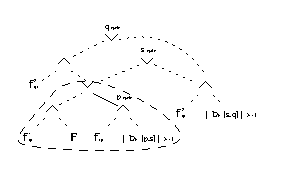
\includegraphics[scale=2]{Figure/figure_17} \\ 
%% \footnotesize
%% (a) A code fragment & 
%% \footnotesize (b) Expression tree storing the boolean
%% functions \\ 
%% & \footnotesize generated after {\tt S2}. \\
%%   \end{tabular}
%%   \caption{Scheme to store the boolean functions generated at
%%     each program point}
%% \label{fig:performance_storage}
%% \end{figure}
%% }
}}

%%%%%%%%%%%%%%%%%%%%%%%%%%%%%%%%%%%%%%%%%%%%%%%%%%%%%
\subsection{Comparison with a Field Insensitive Approach}
%%%%%%%%%%%%%%%%%%%%%%%%%%%%%%%%%%%%%%%%%%%%%%%%%%%%%

For comparison purpose the test cases must involve shape
transitions like Cycle to DAG, Cycle to Tree, and DAG to
Tree. The transition like Tree to DAG, DAG to Cycle, or Tree
to Cycle are not of much importance as these can be detected
by any of the field insensitive approaches. Following are the
cases that meet our requirement and better demonstrate the
accuracy of our analysis as compared to field insensitive
analysis (like Ghiya et.~al.~\cite{Ghiya96}).

\newcommand{\on}{p} 
\newcommand{\nn}{r}

\begin{figure*}[t]
\centering
\scalebox{0.80}{
\begin{tabular}{@{}ll@{}}
  {\small\tt
    \begin{tabular}[b]{l}
      S1. \on$\rightarrow$f = q; \\
      S2. \nn = malloc(); \\
      S3. \nn$\rightarrow$f = q;  \\
      S4. \on$\rightarrow$f = \nn;  
    \end{tabular}
  } &
  \scalebox{0.80}{
    \begin{tabular}[b]{|c||c|c|c|}
      \hline
          {\bf After} & Actual Shape & Field Insensitive
          Analysis & Field Sensitive Analysis \\ 
          \hline \hline
	  {\tt S1}       & Tree		  & Tree    & Tree \\ \hline
	  {\tt S2}       & Tree		  & Tree    & Tree \\ \hline
	  {\tt S3}       & Tree		  & Tree    & Tree \\ \hline
	  {\tt S4}       & Tree		  & DAG(at {\tt \on})    & Tree \\ \hline
    \end{tabular}
  } \\
  \multicolumn{2}{c}{\scalebox{1.00}{(a) Insertion of an
      internal node in a singly linked list }} \\ \\
  {\small\tt
    \begin{tabular}[b]{l}
      S1. n1 = p$\rightarrow$f; \\
      S2. n2 = n1$\rightarrow$f; \\
      S3. t  = n2$\rightarrow$f; \\
      S4. n2$\rightarrow$f = n1; \\
      S5. n1$\rightarrow$f = t; \\
      S6. p$\rightarrow$f = n2;
    \end{tabular}
  } &
  \scalebox{0.80}{
    \begin{tabular}[b]{|c||c|c|c|}
      \hline
          {\bf After} & Actual Shape & Field Insensitive
          Analysis & Field Sensitive Analysis \\ 
          \hline \hline
          {\tt S1}       & Tree		  & Tree                       & Tree \\ \hline
          {\tt S2}       & Tree		  & Tree                       & Tree \\ \hline
	  {\tt S3}       & Tree		  & Tree                       & Tree \\ \hline
	  {\tt S4}       & Cycle (at {\tt p}, {\tt n1}, {\tt n2}) 	   & Cycle (at {\tt p}, {\tt n1}, {\tt n2}) & Cycle (at {\tt p}, {\tt n1}, {\tt n2}) \\ \hline
	  {\tt S5}       & Tree		  & Cycle (at {\tt p}, {\tt n1}, {\tt n2})                       & Tree \\ \hline
	  {\tt S6}       & Tree		  & Cycle (at {\tt p}, {\tt n1}, {\tt n2})                       & Tree \\ \hline
    \end{tabular}
  } \\
  \multicolumn{2}{c}{\scalebox{1.00}{(b) Swapping two nodes
      of a singly linked list}} \\ \\
  {\small \tt
    \begin{tabular}[b]{l}
      mirror(tree T) \{ \\
      S1.    L  = T->left; \\
      S2.    R = T->right; \\
      S3.    mirror(L); \\
      S4.    mirror(R); \\
      S5.    T->left = R; \\
      S6.    T->right = L; \\
      \}  
    \end{tabular}
  } &
  \scalebox{0.80}{
    \begin{tabular}[b]{|c||c|c|c|}
      \hline
          {\bf After} & Actual Shape & Field Insensitive
          Analysis & Field Sensitive Analysis \\ 
          \hline \hline
	  {\tt S1}       & Tree		  & Tree    & Tree \\ \hline
	  {\tt S2}       & Tree		  & Tree    & Tree \\ \hline
	  {\tt S5}       & Dag (at T)	  & Dag (at T)    & Dag (at T) \\ \hline
	  {\tt S6}       & Tree		  & Dag (at T)    & Tree \\ \hline
    \end{tabular}
  } \\
  \multicolumn{2}{c}{\scalebox{1.00}{(c) Computing mirror
      image of a  binary tree.}}
\end{tabular}}
\caption{Examples demonstrating the preciseness of our analysis\label{fig:benchmark_2}}
\end{figure*}

\begin{itemize}
%%%%%%%%%%%%%%%%%%%%%%%%%%%%%%%%%%%%%%%%%%%%%%%%%%%%%
\item[(a)] {\bf Inserting an internal node in a singly linked
  list: }
%%%%%%%%%%%%%%%%%%%%%%%%%%%%%%%%%%%%%%%%%%%%%%%%%%%%%
Consider the code fragment Fig.~\ref{fig:benchmark_2}(a) that
is a simplified version of insertion of an internal node in a
linked list.  Field insensitive approach like that of Ghiya
et.~al.~\cite{Ghiya96} cannot detect the kill information due
to the change of the field $f$ of {\tt \on} at {\tt S4} and
finds {\tt \on} to have an additional path to $\q$ via {\tt
  \nn} (which is now actually the only path). So they report
the shape attribute of {\tt \on} as DAG.

Consider the following boolean function generated after {\tt
  S4} using our approach.
\begin{eqnarray*}
  \on_{\subD} &=&   (f_{\on\q} \wedge (\num{I_F[\on\q]} > 1)) 
  \vee  (f_{\on\nn} \wedge (\num{I_F[\on\nn]} > 1)) \\
  f_{\on\nn} &=& \true \qquad\qquad  f_{\on\q} = \false
\end{eqnarray*}
After {\tt S4}, the condition $\num{I_F[\on,\nn]} > 1$ become
\false\ and $\on_{\subD}$ will get evaluated to \false, and
thus correctly detects the shape attribute of {\tt \on} to
tree.
%%%%%%%%%%%%%%%%%%%%%%%%%%%%%%%%%%%%%%%%%%%%%%%%%%%%%
\item[(b)] {\bf Swapping two nodes of a singly linked list: }
%%%%%%%%%%%%%%%%%%%%%%%%%%%%%%%%%%%%%%%%%%%%%%%%%%%%%
Consider the code fragment Fig.~\ref{fig:benchmark_2}(b)
which swaps the two pointers $p$ and $p\rightarrow f$ in a
singly linked list $L$ with link field as $f$, given the
pointer $p$. The table in Fig.~\ref{fig:benchmark_2}(b) shows the
comparison between the shape decision given by our approach
and the field insensitive approaches.
%%%%%%%%%%%%%%%%%%%%%%%%%%%%%%%%%%%%%%%%%%%%%%%%%%%%%
\item [(c)]{\bf Computing mirror image of a  binary tree: }
%%%%%%%%%%%%%%%%%%%%%%%%%%%%%%%%%%%%%%%%%%%%%%%%%%%%%
Consider the code fragment Fig.~\ref{fig:benchmark_2}(c)
which creates a mirror image of a binary tree rooted at
$T$. While swapping the left and right sub-tree a temporary
DAG is created (after statement {\tt S6}), which gets
destroyed after the very next statement {\tt S7}. As depicted
in Fig.~\ref{fig:benchmark_2}(c), this shape transition is also
captured in our analysis.
\end{itemize}

%%%%%%%%%%%%%%%%%%%%%%%%%%%%%%%%%%%%%%%%%%%%%%%%%%%%%
\section{Conclusion and Future Work} \label{sec:concl}
%%%%%%%%%%%%%%%%%%%%%%%%%%%%%%%%%%%%%%%%%%%%%%%%%%%%%

In this paper we proposed a field sensitive shape analysis
technique. We demonstrated how boolean functions along with
field sensitive matrices help in inferring the precise shape
of the data structure.  While field sensitive matrices help
in generating the kill information for strong updates,
boolean functions help in remembering the shape transition
history with respect to each heap-directed pointer. We have
shown some example scenarios that can be handled more
precisely by our analysis as compared to an existing field
insensitive analysis. Our shape analysis can be utilized by
an optimizing compiler to disambiguate memory references.

%%Our analysis is mainly intra procedural.  
We use a very simple inter procedural framework to handle
function calls, that computes safe approximate summaries to
reach fix point .  Our next challenge is to develop a better
inter procedural analysis to handle function calls more
precisely. Further, we plan to extend our shape analysis
technique to handle more of frequently occurring programming
patterns to find precise shape for these patterns. \hide{{ We
    also want to improve our summarization technique. Earlier
    we have used graph based approximations of access
    paths~\cite{khedker07heap} to compute liveness of heap
    data. We plan to explore if the same summarization
    technique can also be applied here instead of
    $k$-limiting.}} We are developing a prototype model using
GCC framework to show the effectiveness on large
benchmarks. However, this work is still in very early stages,
and requires manual intervention. We plan to automate the
prototype in near future.

\bibliographystyle{abbrv}
\bibliography{sigproc}  

\end{document}
